\documentclass{article}

\usepackage[T1]{fontenc}
\usepackage[utf8]{inputenc}
\usepackage[swedish]{babel}
\usepackage{fullpage}
\usepackage{amssymb}
\usepackage{bussproofs}
\usepackage{amsmath}
\usepackage{wrapfig}
\usepackage{float}
\usepackage{graphicx}
\usepackage{verbatim}
\usepackage{tikz}
\let\emptyset\varnothing


\title{Supplemental Instructions}
\author{Benjamin Eriksson \& Erik Thorsell \\ 
		\small{beneri@student.chalmers.se} \&
		\small{erithor@student.chalmers.se}
}
\date{
      2015-02-24
     }

\begin{document}
\maketitle
%UPPGIFT 1%
\subsection*{1}
Använd Trapzeoidregeln för att approximera $\int_0^{\pi} sin(x) dx$
\begin{itemize}
    \item[a) ] med 10 subintervall.
    \item[b) ] med 20 subintervall.
\end{itemize}   

%UPPGIFT 2%
\subsection*{2}
{\it Gå till sida 397!}\\
$S$ fås genom att snurra det område som avgränsas av $y = x^2$ 
runt $x$-axeln. Vad är S volym om området även begränsas av $y = 0$ och 
$x = 1$ och: 
\begin{itemize}
    \item[a) ] du använder diskmodellen?
    \item[b) ] du använder skalmodellen?
\end{itemize}

%UPPGIFT 3%
\subsection*{3}
Beräkna längden av följande kurvor: \\
\begin{itemize}
	\item[a) ] $y = \frac{4}{3} \> x$, där x går från 0 till 3.
	\item[b) ] $y = \frac{2}{3} (x-1)^{ \frac{3}{2} }$, där x går från 0 till 4. 
\end{itemize}





%UPPGIFT 4%
\subsection*{4}
Området begränsat av $x$-axeln och kurvan $y=x(2-x)$ roteras kring $x$-axeln. 
Beräkna resulterande volym.\\
{\emph Tentamen 20140114}

\begin{wrapfigure}{r}{0.3\textwidth}
  \begin{center}
    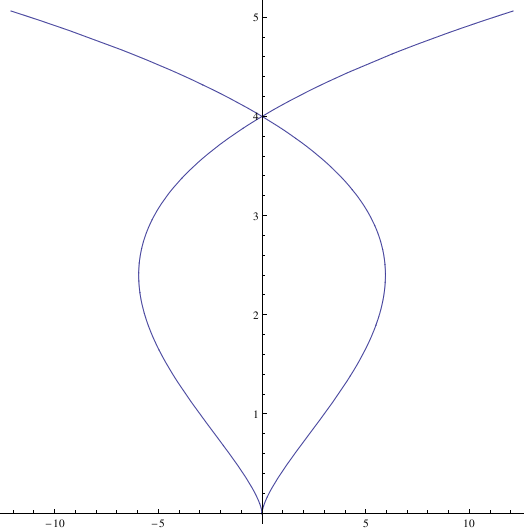
\includegraphics[width=0.3\textwidth]{curve}
  \end{center}
\end{wrapfigure}

%UPPGIFT 5%
\subsection*{5 Parametriserade kurvor}
Den parametriska kurva nedan är definerad som: \\
$x = t^5 - 4t^3$   \\
$y = t^2$ \\
Hitta tangenten vid x = 0, y = 4.





\end{document}
